\documentclass[/Users/ikedahajime/GitHub/reserch/master_report/thesis]{subfiles}
% このファイル内だけのコマンド
\begin{document}
\chapter{手法と数値計算設定}
この章ではシミュレーションの設定と、計測したパラメータについて記す。
\section{数値シミュレーションの設定}
% \cite{filyAthermalPhaseSeparation2012}
\secref{sec:result_abp}では inertial inertial Active Brownian Particles(iABP) モデルを用いた。
iABP モデルは以下のように表される。
% ABPの方程式
\begin{eqnarray}
    \dot{\bm{v}_i}(t)&=& - \zeta \bm{v}_i  +\bm{F}_i +\zeta v_0 \bm{e}(\theta_i(t))
    % \dot{\bm{r}_i}(t) &=& \zeta \bm{F}_i(t)+v_0 \bm{e}(\theta_i (t))
\end{eqnarray}
\begin{eqnarray}
    \dot{\theta_i }(t) &=& \sqrt{\frac{2}{\tau}}\eta_i(t)
\end{eqnarray}
ここで、\mbox{\boldmath$r$}は粒子の位置、$v_0$ は自己推進の速度、$\zeta$ は摩擦係数を表す。
$\eta_i$ はホワイトノイズで、$\langle \eta_i(t) \eta_j(t') \rangle=\delta_{ij}\delta(t-t')$の関係を満たす。
ここで、$\langle \dots \rangle$ はアンサンブル平均である。
$\mbox{\boldmath$e$}(\theta_i)=(\cos\theta_i,\sin \theta_i)$は自己推進の方向を表す単位ベクトルで、
$\tau$は緩和時間である。このモデルは、各粒子が角度$\theta_i$の方向に、持続時間$\tau$の間、速度$v_0$で進むことを表す。


$\bm{F}_i$は相互作用を表し、二体間相互作用ポテンシャル$U(r)$と壁との相互作用$\bm{F}_{wall}$を用いて
$\bm{F}_i=-\sum_{i\neq j} \bm{\nabla}_iU(r_{ij})+c_{wall}\bm{F}_{wall}$と書ける。$c_{wall}$は壁による
力の大きさを表す定数で、ここでは1にとった。
ポテンシャルには、Weeks-Chandler-Andersen(WCA)ポテンシャル\cite{weeksRoleRepulsiveForces1971}を用いた。
\begin{equation}
    U(r_{ij})=
    \begin{cases}
        4\epsilon\left(\left(\frac{\sigma}{r_{ij}}\right)^{12}-\left(\frac{\sigma}{r_{ij}}\right)^6+\frac{1}{4}\right) & (r_{ij}<2^{\frac{1}{6}}\sigma)\\
        0 &(r_{ij}>2^{\frac{1}{6}}\sigma)
    \end{cases}
\end{equation}
ここで、$r_{ij}=\left|\bm{r}_i-\bm{r}_j\right|$は粒子間距離、$\sigma$は粒径、$\epsilon$は相互作用の強度である。
本研究では粒子を閉じ込める壁を\figref{fig:setup_circles}のように取る。壁との相互作用には同じポテンシャルを用い、壁による力は
$\bm{F}_{wall}=-\bm{\nabla}U(r_{wall})$と表される。
$r_{wall}$は壁と粒子の距離を表し、$\bm{r}_c$を円の中心をさすベクトルとして$r_{wall}=R+0.5\sigma-\left|\bm{r}-\bm{r}_c\right|$
と表される。


\begin{figure}
    \centering
    \begin{tabular}{c}
        \begin{minipage}{0.2\hsize}
            % \text{(a)}
            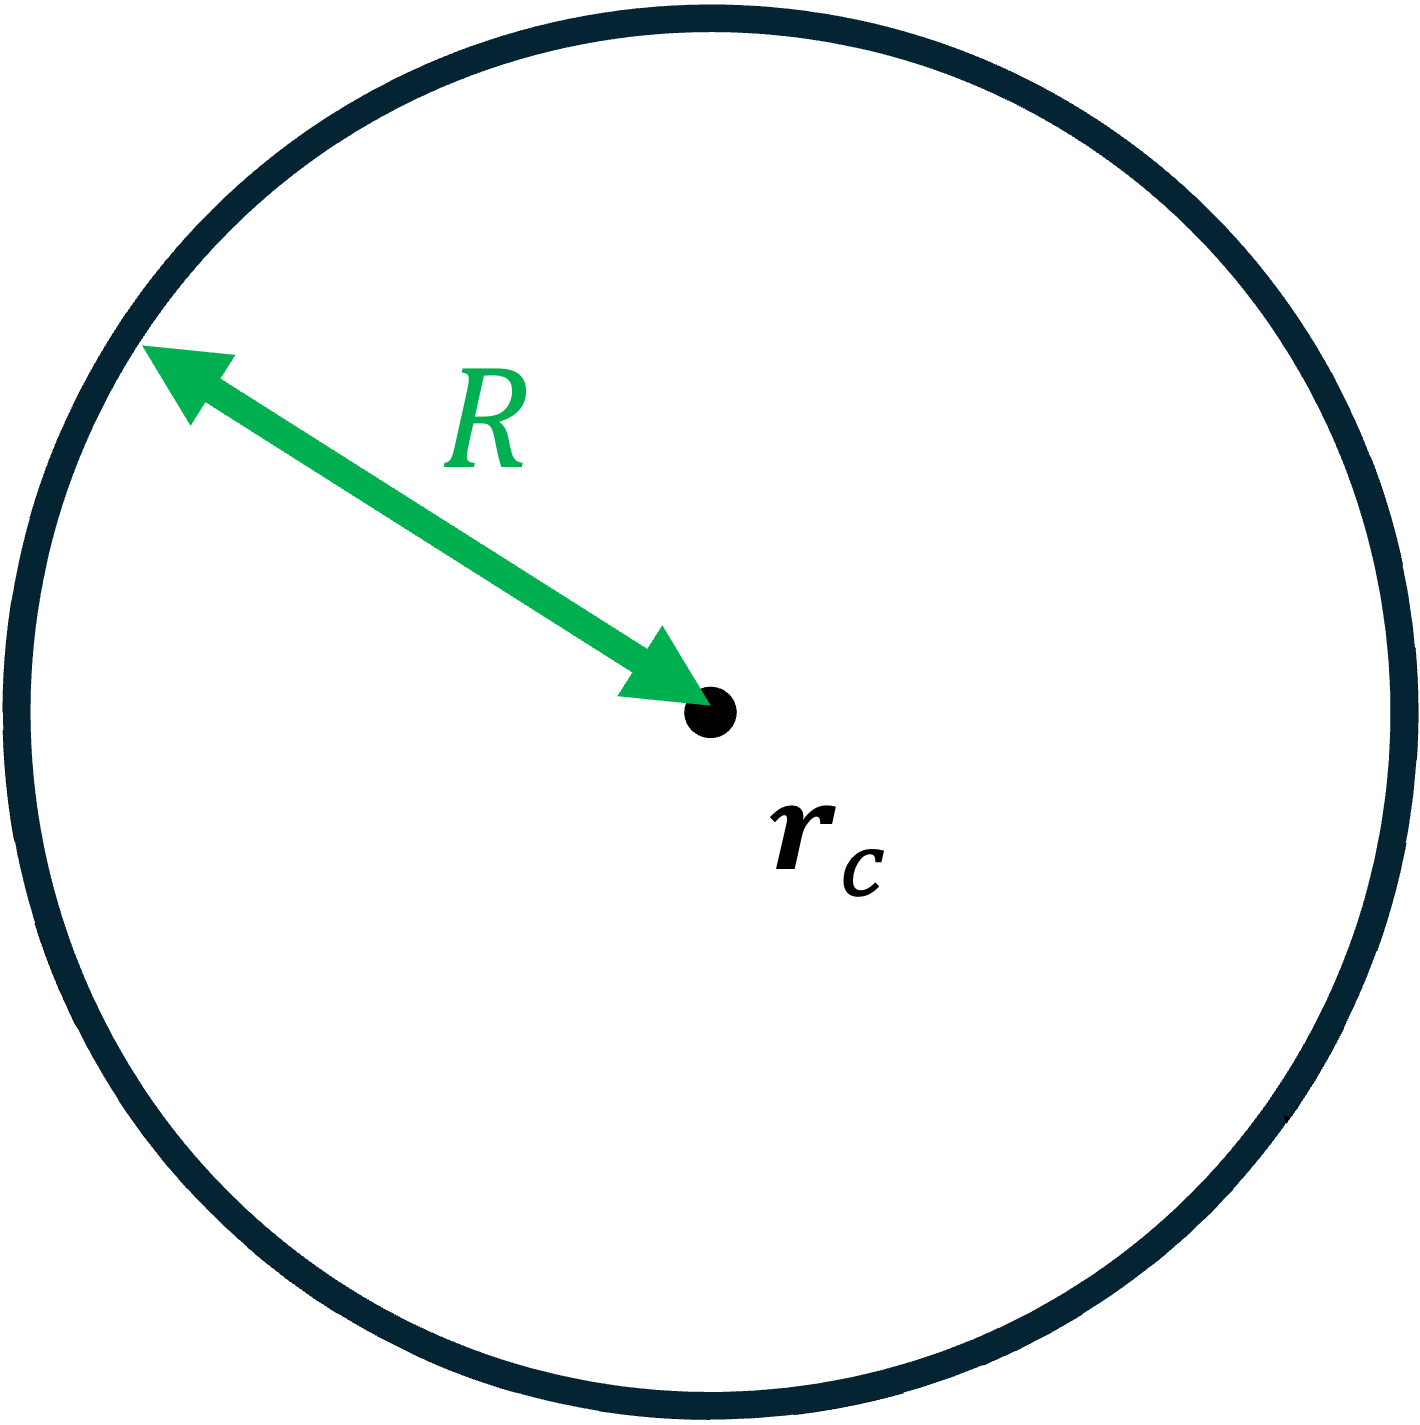
\includegraphics[width=\textwidth]{img/method/fig_sincer.png}
        \end{minipage}
    \end{tabular}
    \caption[fig:circle]
    {
        円が1つの系の壁に関する模式図。
    }
    \label{fig:setup_circles}
\end{figure}
数値計算のため、長さの単位を$\sigma$、時間の単位を$\sigma/v_0$と置いた。無次元化した質量$M=mv_0/\zeta\sigma$、
 Péclet 数$Pe=v_0\tau/\sigma$、エネルギーと速度の比$\epsilon^*=\epsilon/\sigma v_0 \zeta$
をパラメータに取り、このうち$\epsilon^*=1$とした。
粒子数$N$は、面積分率$\varphi$と系の面積$S$を用いて$N=4\varphi S/\pi\sigma^2$とした。
コントロールパラメータとして、系の半径$R、Pe、M、\varphi$を用いた。


% コントロールパラメータは、
\secref{sec:result_cabp}では、ABPにキラリティーに関する項を加えた、 Chiral Active Brownian Particles(CABP)%\cite{teeffelenDynamicsBrownianCircle2008}%TODO::aliment forceがないものに変える
を用いた。このモデルは以下のように表される。
% CABPの方程式
\begin{eqnarray}
    \dot{\bm{r}_i}(t) &=& \frac{1}{\zeta} \bm{F}_i(t)+v_0 \bm{e}(\theta_i (t))
\end{eqnarray}
\begin{eqnarray}
    \dot{\theta_i }(t) &=& \Omega+\sqrt{\frac{2}{\tau}}\eta_i(t)
\end{eqnarray}
ここで、$\Omega$はキラリティーの強度である。

ポテンシャルにはHarmonicポテンシャルを用いた。
\begin{equation}
    U(r_{ij})=
    \begin{cases}
        \frac{\epsilon}{2}\left(\frac{r_{ij}}{\sigma}-1\right)^2 &(r_{ij}<\sigma)\\
        0 & (r_{ij}>\sigma)

    \end{cases}
\end{equation}
壁との相互作用には同様にHarmonicポテンシャルを用い、力の大きさを表す定数$c_{wall}=100$とした。


本研究では最も簡単な場合として揺らぎがゼロ、つまり緩和時間$\tau=\infty$の極限を解析した。
$\epsilon^*=40$に固定し、コントロールパラメータとして系の半径$R$、粒子の回転半径$R_\Omega=v_0/\Omega$、面積分率$\varphi$を用いた。


\section{オーダーパラメータ}
観測するパラメータとして、以下のパラメータを用いた。
\subsection{渦秩序変数}\label{subsec:vortes_order_parameter}
系が渦をなしているかどうかを定量化するために、
渦秩序変数$\psi$\cite{wiolandConfinementStabilizesBacterial2013}を以下のように定義する。
\begin{equation}
    \psi=\frac{\sum_i \left|\bm{v}_i\cdot \bm{t}_i \right|/\sum_i v_i -2/\pi}{1-2/\pi}
\end{equation}
ここで、$\bm{t}_i$は角度方向の単位ベクトルである。$\psi>0$の時は角度方向の流れが、$\psi<0$の時は動系方向の流れが生じていることがわかる。
特に$\psi\simeq1$の時全ての粒子が角度方向に運動していることを、$\psi\simeq0$の時無秩序な流れが生じていることを示す。


\subsection{規格化された角運動量}
本研究では高密度系でのシミュレーションを行う。この場合、粒子は動径方向の運動をほとんど行わず、角度方向の
運動が支配的になる。そのため\subsecref{subsec:vortes_order_parameter}で定義した渦秩序変数のように
動径方向の運動を考慮したオーダーパラメータを使う必要がない。また、渦秩序変数は渦の回転方向に関する情報を得ることができない。
そこで、以下のように定義される規格化された角運動量$V$\cite{jiangEmergenceCollectiveDynamical2017,capriniCollectiveEffectsConfined2021}を用いる。
\begin{equation}
    V=\frac{1}{N} \sum_i \frac{L_{zi}}{ |L_{zi}|}
\end{equation}
ここで、$L_{zi}$は$i$番目の粒子の角運動量で、$L_{zi}=x_i*v_{yi}-y_i*v_{xi}$。


このパラメータは、角度方向の運動方向が揃っているか、及びその回転方向がどちらかを判定するパラメータである。
まず絶対値に注目すると、絶対値が小さいとき、つまり$|V|\simeq 0$のとき、時計回り、反時計回りに運動する粒子が同数存在し、
系全体での渦が生じていないことが分かる。
反対に絶対値が大きいとき、つまり$|V|\simeq 1$のときは系全体が原点を中心とした一つの渦をなして一方向に回っていることが分かる。


続いて、$|V|\simeq 1$として、その正負について考える。すると、値が負、つまり$V\simeq -1$のときは時計回りの渦が、
値が正、つまり$V\simeq 1$のときは反時計回りの渦が発生していることを読み取ることができる。


\subsection{渦度}\label{subsec:def_vortex}
渦度場は、速度場$\bm{v}(\bm{r})$を用いて$\omega(\bm{r})=\partial_x v_y -\partial_y v_x$と表される。
数値計算上、速度場は以下のように計算する。空間を$\delta x=\delta y=0.25 \sigma$の格子状に分割する。
このとき、格子点$r(i,j)$における速度場は%この書き方でいいのか?
\begin{equation}\label{eq:valocity_field}
    \bm{v}(r(i,j))=\sum_{\left|\bm{r}_k-r(i,j)\right|<3\sigma} f(\left|\bm{r}_k-r(i,j)\right|)\bm{v}_k
\end{equation}
のように計算する。ここで、$f(r)=(2\pi s^2)^{-1} \exp(-r^2/2s^2)$はガウシアン関数であり、分散$s$は$3/\sqrt{2\log 10}$とした。


この速度場を用いて、渦度場は格子点の周りの速度場を線積分することで計算される。
\begin{equation}
    \omega (r(i,j))=\frac{v_x(r(i,j))\delta x +v_y(r(i+1,j)) \delta y -v_x(r(i+1,j+1))\delta x -v_y(r(i,j+1))}{\delta x \delta y}
\end{equation}

\subsection{方位角成分の運動量}
円の中に生じる渦の定量化のため、方位角成分の運動量を導入する\cite{nishiguchiVortexReversalPrecursor2024}。
この量は円の中に複数の渦があることを示す量であり、$m_n$は$2n$個の渦があることを表す。
方位角成分の運動量は以下のように定義される。
\begin{eqnarray}
    m_n &=& \int_0^R dr r\left|\frac{1}{2\pi}\int_0^{2\pi}d\theta \bm{v}(r,\theta)\right|^2
\end{eqnarray}
ここで、$\bm{v}(r,\theta)$は極座標系の速度場である。
数値計算する際には、\subsecref{subsec:def_vortex}と同様に式\eqref{eq:valocity_field}に基づいて求めた速度場を使用し、
積分計算には幅0.25の中点法を用いた。
ただし、ここで用いる速度場では格子点を$x$軸、$y$軸共に格子の半分$\delta x/2=\delta y/2=0.125$だけ平行移動して計算した。

\subsection{結晶秩序変数}
結晶化について議論するためのオーダーパラメータの1つに結晶秩序変数$\phi_6$がある。
このパラメータは系が結晶構造をなしているかを表す物理量で、以下のように定義される。
本研究では、一粒子に対するパラメータ$\phi_{6j}$を用いる。
\begin{equation}
    \phi_{6j}=\frac{1}{6}\sum_{k\in \mathcal{N}_{6j}} e^{6i\theta_{jk}}
\end{equation}
ここで、$\mathcal{N}_{6j}$は$j$番目の粒子の6つの最近説粒子を、$\theta_{jk}$は
ベクトル$\bm{r}_j-\bm{r}_k$がx軸となす角度である。

\end{document}
